%---------change this every homework
% place your email id between the braces so that your homework has a name
\def\yourname{Hamlet}
% -----------------------------------------------------
\def\homework{1} % 0 for solution, 1 for problem-set only
\def\duedate{Friday, February 26 at 5pm}
\def\duelocation{via \href{https://www.gradescope.com/courses/80616/}{gradescope}}
\def\hnumber{5}
\def\prof{Andrew Drucker, Lorenzo Orecchia}
\def\course{\href{https://canvas.uchicago.edu/courses/25977}{CMSC 27200 - Winter 2021}}
%-------------------------------------

\documentclass[10pt]{article}
\usepackage[colorlinks,urlcolor=blue]{hyperref}
\usepackage[osf]{mathpazo}
\usepackage{amsmath,amsfonts,graphicx,amsthm}
\usepackage{algpseudocode}
\usepackage{tikz}
\usepackage{latexsym}
\usepackage{subfig}
\usepackage{enumitem}
\usepackage{listings}
\usepackage{fullpage}
\usepackage{color}
\definecolor{mdb}{rgb}{0.3,0.02,0.02} 
\definecolor{cit}{rgb}{0.05,0.2,0.45} 
\markboth{\yourname}{\yourname}
\theoremstyle{definition}

\newcommand{\alg}[1]{\mathsf{#1}}
\newcommand{\handout}{
   \renewcommand{\thepage}{H\hnumber-\arabic{page}}
   \noindent
   \begin{center}
      \vbox{
    \hbox to \columnwidth {\sc{\course} --- \prof \hfill}
    \vspace{-2mm}
    \hbox to \columnwidth {\sc due \MakeLowercase{\duedate} \duelocation\hfill {\Huge\color{mdb}H\hnumber.\yourname}}
      }
   \end{center}
   \vspace*{2mm}
}
\newcommand{\solution}[1]{\medskip\noindent{\color{cit}\textbf{Solution:} #1}}

\newcommand{\bit}[1]{\{0,1\}^{ #1 }}
\newtheorem{problem}{\sc\color{cit}Problem}
\newtheorem{lemma}{Lemma}
\newtheorem{theorem}{Theorem}
\newtheorem{definition}{Definition}
\newtheorem{claim}{Claim}

\setlength{\parskip}{1em}

\begin{document}
\handout
\begin{itemize}
\item The assignment is due on Gradescope on Friday, February 26 at 5pm. 

\item You can either type your homework using \LaTeX~or scan your handwritten work. We will provide a \LaTeX~template for each homework. If you writing by hand, please fill in the solutions in this template, inserting additional sheets as necessary. This will facilitate the grading.

\item You are permitted to discuss the problems with up to 2 other students in the class (per problem); however, {\em you must write up your own solutions, in your own words}. Do not submit anything you cannot explain. If you do collaborate with any of the other students on any problem, please do list all your collaborators in your submission for each problem. 

\item Similarly, please list any other source you have used for each problem, including other textbooks or websites.


\item {\em Show your work.} Answers without justification will be given little credit.
\end{itemize}

%%%%%%%%%%%%%%%%%%%%%%%%%%%%%%%%%%%%%%%%%%%
% PROBLEM 1
%%%%%%%%%%%%%%%%%%%%%%%%%%%%%%%%%%%%%%%%%%%
\newpage
\begin{problem}[35 points]
NASA's Perseverance Rover has just landed on Mars! You are the scientist now in charge of navigating the rover as it visits locations on the Martian surface to perform experiments. The region that the rover has landed in is modeled as a topographical map represented by an $N \times N$ grid. For each point $(i, j)$, there is an associated \textbf{height} $h_{i,j} \geq 0$ and \textbf{scientific value} $v_{i,j}$ for visiting the location. 

Because we want the rover to run as long as possible, you are also required to conserve energy during navigation and are subsequently \emph{forbidden from moving the rover uphill}. The Rover's movements can thus be summarized as follows. The rover starts at position $\big( \frac{N}{2}, \frac{N}{2} \big)$ and is allowed to navigate from positions $(i, j)$ to $(i', j')$ where $i' = i \pm 1$ and $j' = j \pm 1$ provided that $h_{i',j'} \leq h_{i, j}$. Image surveys determine that nothing outside the grid is reachable -- you may treat this boundary as having $h_{ij} = +\infty$.

Subject to these constraints, construct an algorithm that outputs a path, represented as a sequence of $(i, j)$, that maximizes the sum of scientific values in Perseverance’s journey. Prove that your algorithm is correct, and that it runs in polynomial time with respect to $N$. In your running time analysis, provide an explicit $O(\cdot)$ bound.
\end{problem}
\solution{
\paragraph{} collaborated with Yael Sulkin

\begin{algorithmic}
    \State Let P be the array of reachable values defined as $(i,j) \cup {(i+1,j), (i, j+1), (i-1,j), (i,j-1)}$
    \While P is not empty
        \State Move to value with max height ($h_{i',j'}$) and/or max value ($v_{i',j'}$) such that $(i,j) \Leftarrow i',j'$ where $h_{i',j'} \leq h_{i,j}$
        \State If all surrounding values are of the same height, choose the one with best value. 
    \If {$h_{i',j'} < h_{i,j}$}
        \State remove $i,j$ from P
        \State add $i,j$ to array K
    \EndIf
    \EndWhile
        \State Return K 
\end{algorithmic}

\paragraph{Proof of Runtime} Our algorithm may visit locations more than once if the heights are the same but values are not recounted. 
Let's assume all heights are distinct thus the perseverance rover will only ever travel to positions once, as once it moves to a lower height
the past height is removed from the array of reachable positions. Traveling to all points once from starting position to the lowest position 
gives a time complexity of $O(N)$. 

\paragraph{Proof of Correctness} We will solve this problem using Dynamic programming where we want to 
establish a subfamily of $k*k$ points within $N*N$ where $k < N$. So, let our input array be $A_m = 
{p_1, p_2, p_3, \ldots p_n}$ where $m \leq n \leq N*N$ and $p_m$ stands for position $(i,j)$ at the mth index
in the 2D array. Let our Output array K be the sequence of positions $(i,j)$ in order which maximize the 
scientific values that can be reached. Let $J \subseteq [n]$ and we want to maximize the sum of values 
for J, denoted as $V(J)$. Our subproblem will maintain the same goal as our problem but also $J \subseteq 
[k], k < n$ where J is "k-restricted". Next we want to establish the k'th subfamily. 

\subparagraph{Defining Solutions} Let $OPT_k$ define the solution for our subproblem and let $OPT_n$ be 
the optimal solution. We can establish our base case at our first position $(\frac{N}{2}, \frac{N}{2})$
where $V(K) = OPT_k = V(N) = OPT_n = v_{\frac{N}{2}, \frac{N}{2}}.$ We want to define $OPT_{k+1}$ so we 
can work towards $OPT_n$ from $OPT_k$. We claim that $1 < k < n$, $OPT_{k+1} /geq max\{OPT_k, v_{k+1} + OPT_l\}$
where $l = max\{j \leq k, v_j \leq v_k+1\}$ In other words, we want to establish that $OPT_{k+1}$ will always be at 
least $OPT_k$ or can be included in a subset of $OPT_k, OPT_l$ where the next position $p_{k+1}$ with value $v_{k+1}$ 
can be reached. 

\subparagraph{} We want to show that $OPT_{k+1} \geq OPT_k$

\subparagraph{} We want to show that $OPT_{k+1} \geq v_{k+1} + OPT_l$

\paragraph{} Thus our final sequence obeys the same bases cases and recurrences of our $OPT_k$ family so by 
principle of induction $OPT_k$ and $OPT_n$ are equal. 


  Your solution goes here.
}

\newpage
\medskip\noindent{\color{cit} Extra Space for your solution}

%%%%%%%%%%%%%%%%%%%%%%%%%%%%%%%%%%%%%%%%%%%
% PROBLEM 2
%%%%%%%%%%%%%%%%%%%%%%%%%%%%%%%%%%%%%%%%%%%
\newpage
\begin{problem}[30 points]
In this exercise, we explore the effect of perturbations on the capacity of a single edge on the value of the maximum flow in a flow network with integral capacities. Consider the following types of edges in a flow network.
\begin{itemize}
\item An edge of a flow network is called {\bf critical} if decreasing the capacity of this edge results in a decrease in the maximum flow.

\item An edge of a flow network is called a {\bf bottleneck} edge if increasing its capacity results in an increase in the maximum flow.
\end{itemize}

Given a flow network $G = (V, E)$ with integer capacities $c_e \geq 0$, prove or provide a counterexample for each of the following statements.
\begin{enumerate}[label=(\alph*),leftmargin=2\parindent]
\item All critical edges are bottleneck edges.

\item A critical edge always exists.

\item A bottleneck edge always exists.
\end{enumerate}
\end{problem}

\solution{
\paragraph{} collaborated with Yael Sulkin

\paragraph{A} This claim is false and the folowing example will help prove why:

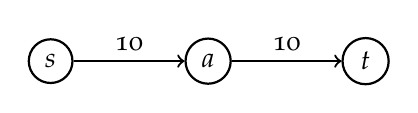
\begin{tikzpicture}[node distance={20mm}, thick, main/.style = {draw, circle}] 
    \node[main] (1) {$s$};
    \node[main] (2) [right of=1] {$a$};
    \node[main] (3) [right of=2] {$t$};
    \draw[->] (1) -- node[midway, above] {10} (2);
    \draw[->] (2) -- node[midway, above] {10} (3);
  \end{tikzpicture} 

  The reason why all critical edges are not always bottleneck edges is because of the conservation of flow. 
  In the above case both edges $e_{sa}, e_{at}$ are critical edges because the max amount of flow at either edge is 10. If 
  the capacity of $e_{sa}$ were to decrease to 7 then the max flow would be 7 and because of conservation of flow, edge $e_{at}$
  would also have a flow of 7 (even with a capacity of 10). This is due to the fact that the amount of flow that goes into a
  is exactly the same amount of flow that goes out of a. The reason why these edges are critical and not bottleneck edges is because 
  the conservation of flow in sequence means that two edges require the same amount of flow if there are no other edges leading outwards.
  For example, we could increase edhe $e_{sa}$ to a capacity of 15 but because the capacity of $e_{at}$ is 10, flow can at max be 10. 
  Since flow can only ever be less than capacity, critical edges aren't always bottleneck edges because there could be multiple critical edges. 

\paragraph{MaxFlow MinCut theorem} We can use the MaxFlow MinCut theorem to help explain. From the MaxFlow Mincut theorem we know that 
for a cut $(A,B)$ where $s \in A$ and $t \in B$ the maxFlow $v(f) = \sum f(e)_{out of A} - \sum f(e)_{into A} \leq cap(A,B) = \sum {c_(e)}_{out of A}$. 
We can define a critical edge $c_{e'}$ as $v(f) \leq  \sum {c_(e')}_{out of A} < \sum {c_(e)}_{out of A}$. We can define a bottleneck edge 
$c_{e''}$ as an edge where $\sum {c_(e)}_{out of A} < v(f) \leq  \sum {c_(e'')}_{out of A}$ Thus what our example illustrates is that this can sometimes
not occur when there are multiple edges $e'$ and $e''$ that are needed to connect s and t. 

\paragraph{B} This claim is true because since there always exists a minimum cut there always exists a critical edge. Firstly, we know there 
always exists a minimum cut because of the finite number of nonnegative edges. As follows, if there is a minimum cut there exists an edge 
with minimal capacity of the Graph. 

\paragraph{C} This claim is false, and is supported by the example above part A. The example in part A has 0 bottleneck edges because both 
edges are critical and are both needed to connect $s-t$. Niether edge is a bottleneck edge because if the capacity of either is raised, the
max flow remains the capacity of the minimum edge because by assumption flow, f is always $0 \leq f \leq c_e$ where $c_e$ is the capacity of a 
certain edge. 








  Your solution goes here.
}


\newpage
\medskip\noindent{\color{cit} Extra Space for your solution}

%%%%%%%%%%%%%%%%%%%%%%%%%%%%%%%%%%%%%%%%%%%
% PROBLEM 3
%%%%%%%%%%%%%%%%%%%%%%%%%%%%%%%%%%%%%%%%%%%
\newpage
\begin{problem}[35 points]
In a particular network $G=(V,E)$ whose edges have integer capacities $c_e$, we have already found the maximum flow $f$ from node $s$ to node $t$. However, we now find out that one of the capacity values we used was wrong: for edge $(u, v)$ we used $c_{uv}$ whereas it should have been $c_{uv} - 1$. This is unfortunate because the flow $f$ uses that particular edge at full capacity: $f_{uv} = c_{uv}$. We could redo the flow computation from scratch, but there's a faster way.

Show how a new optimal flow can be computed in $O(\lvert V \rvert + \lvert E \rvert)$ time. Precisely, construct an algorithm that given the following input, produces the following output.
\begin{itemize}
\item Input -- A flow network $G = (V, E)$ with capacities $c_e \geq 0$ for each $e \in E$, a precomputed maximum $s$-$t$ flow $f$, and an edge $(u, v)$ whose capacity is incorrect. 

\item Output -- A new maximum flow $f'$ using capacities $c'_{uv} = c_{uv} - 1$ and  $c'_e = c_e$ for all $e \neq (u,v)$.
\end{itemize}

Prove that your algorithm is correct and runs in $O( \lvert V \rvert + \lvert E \rvert)$ time. Hint: it may be helpful to consider the set of vertices reachable from $u$ in the residual graph.
\end{problem}

\solution{
  Your solution goes here.
}

\newpage
\medskip\noindent{\color{cit} Extra Space for your solution}

\end{document}